\documentclass[10pt]{beamer}

\usetheme{metropolis}
\usepackage{appendixnumberbeamer}

\usepackage{booktabs}
\usepackage[scale=2]{ccicons}

\usepackage{pgfplots}
\usepgfplotslibrary{dateplot}

\usepackage{xspace}
\newcommand{\themename}{\textbf{\textsc{metropolis}}\xspace}

\newcommand{\dark}{
  \setbeamercolor{normal text}{%
    fg=black!2,
    bg=black
  }
  \setbeamercolor{progress bar}{%
    use=alerted text,
    fg=alerted text.fg,
    bg=alerted text.fg!30!black!90
  }
}
\dark
% \metroset{background=dark}
\metroset{titleformat frame=allcaps}

\title{Media Meets Semantic Web}
\subtitle{How the BBC uses DBpedia and Linked Data to Make Connections}
\date{11$^{th}$ June, 2017}
\author{Andreas Müller}
\institute{Technische Universität Berlin}
% \titlegraphic{\hfill\includegraphics[height=1.5cm]{logo.pdf}}

\begin{document}

\maketitle

\begin{frame}{Table of contents}
  \setbeamertemplate{section in toc}[sections numbered]
  \tableofcontents[hideallsubsections]
\end{frame}

% ------------------------------------------------------------------------------
\section{Problem}

\begin{frame}[fragile]{Problem}

  Large amounts of BBC online content: \textsc{\textbf{text}}, \textsc{\textbf{audio}}, \textsc{\textbf{video}}

  Domain specific microsites: \textsc{\textbf{food}}, \textsc{\textbf{gardening}}, \textsc{\textbf{sport}}, etc. ...

  \pause
  \begin{figure}
    \centering
      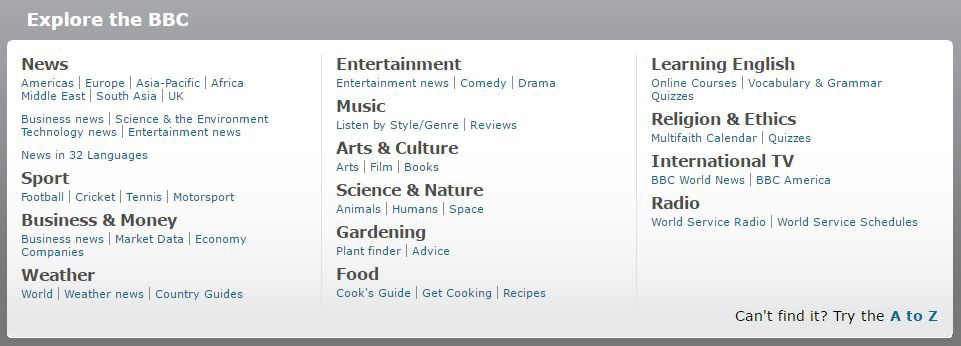
\includegraphics[width=\textwidth]{img/bbc_domains_2009}
    \caption{BBC microsites in June, 2009}
  \end{figure}

\end{frame}

\begin{frame}[fragile]{Problem}

  Large amounts of BBC online content: \textsc{\textbf{text}}, \textsc{\textbf{audio}}, \textsc{\textbf{video}}

  Domain specific microsites: \textsc{\textbf{food}}, \textsc{\textbf{gardening}}, \textsc{\textbf{sport}}, etc. ...

  \begin{figure}
    \centering
      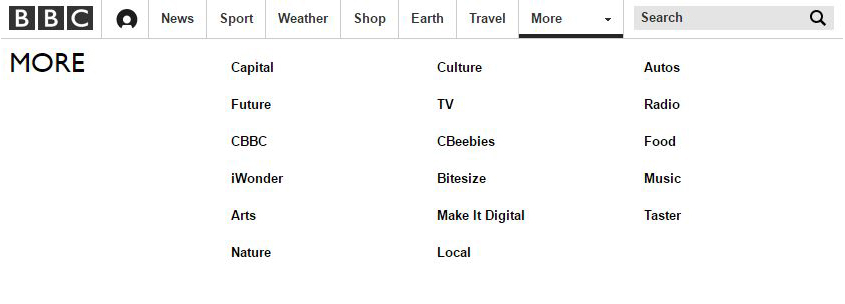
\includegraphics[width=\textwidth]{img/bbc_domains_2017}
    \caption{BBC microsites in June, 2017}
  \end{figure}

\end{frame}

\begin{frame}[fragile]{Problem}

  \alert{\textbf{Not possible to...}}
  \bigskip

  \begin{columns}[T,onlytextwidth]
    \column{0.5\textwidth}
      Find \textbf{everything}, BBC has published to a given subject

    \column{0.5\textwidth}
      Navigate between BBC domains following a \textbf{semantic thread}
  \end{columns}

  \bigskip
  No interlinking between microsites = not using full potential of available data

\end{frame}


% ------------------------------------------------------------------------------
\section{Objectives}

\begin{frame}[fragile]{Objectives}

  Make the BBC website \alert{\textbf{more coherent}} and \alert{\textbf{more useful}}
  \bigskip

  \pause
  Better connections and interlinking of existing systems

  \textbf{Soft transition} and reducing impact on existing systems while adding new services to \textbf{maximize interlinking} of domains

  \pause
  \begin{enumerate}[<+->]
    \item \alert<7>{Service to link all radio and TV programmes}
    \item Develop a new music offering
    \item Retrofit simple navigational elements
    \item \alert<7>{Provide a common set of web scale identifiers}
  \end{enumerate}

\end{frame}


% ------------------------------------------------------------------------------
\section{Interlinking of concepts}

\begin{frame}[fragile]{Interlinking of concepts — CIS}

  Legacy auto-categorization system: {\textbf{CIS}}

  % TODO: image

  \bigskip
  \alert{\textbf{Limits:}}

  \begin{itemize}
    \item Difficult to cover every single entity
    \item No relations between terms are available
    \item Only internal identifiers
  \end{itemize}

\end{frame}

\begin{frame}[fragile]{Interlinking of concepts — DBpedia}

  \begin{columns}[T,onlytextwidth]
    \column{0.5\textwidth}
      Common Vocabulary: {\textbf{DBpedia}}
      \bigskip
      \begin{alertblock}{DBpedia Label Lookup}
        Find most likely matches to a given term, calculate relevance with number of backlinks
      \end{alertblock}

      \begin{alertblock}{Context-based Disambiguation}
        Disambiguate possible matches by clustering them and finding according context in DBpedia
      \end{alertblock}
    \column{0.5\textwidth}
      \begin{figure}
        \centering
          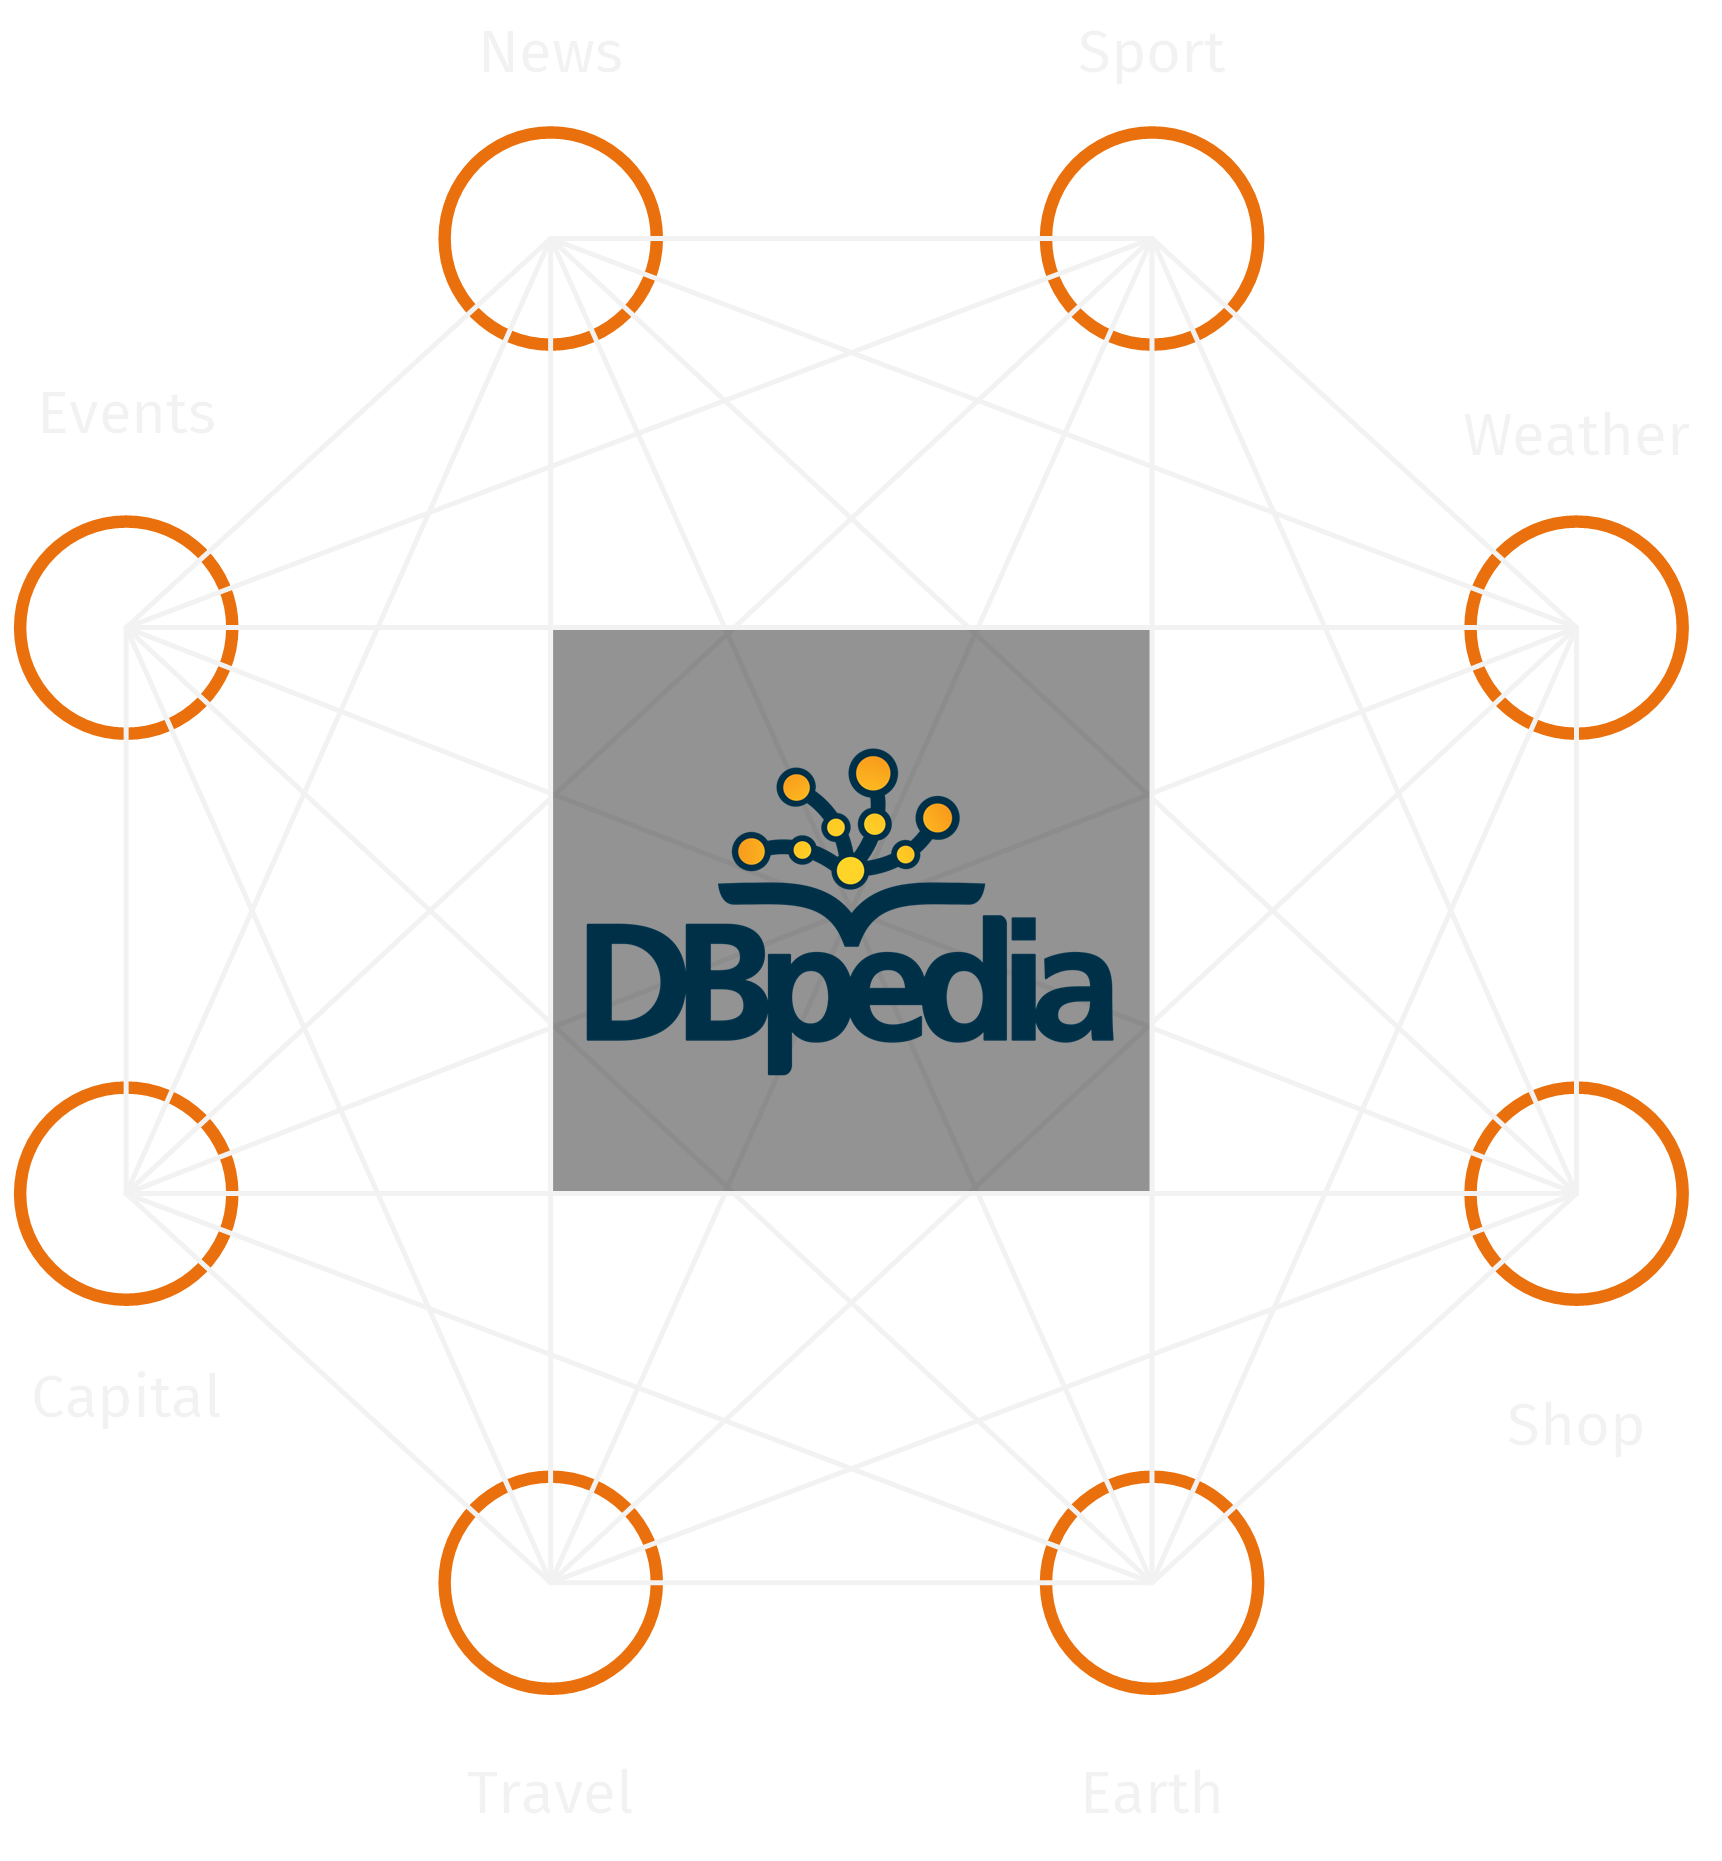
\includegraphics[width=\textwidth]{img/dbpedia.png}
        \caption{Linking BBC Domains}
      \end{figure}

  \end{columns}

\end{frame}


% ------------------------------------------------------------------------------
\section{Interlinking of documents}

\begin{frame}[fragile]{Interlinking of documents — Muddy Boots}

  Identify main actors in a piece of content: {\textbf{Muddy Boots}}

  \begin{figure}
    \centering
      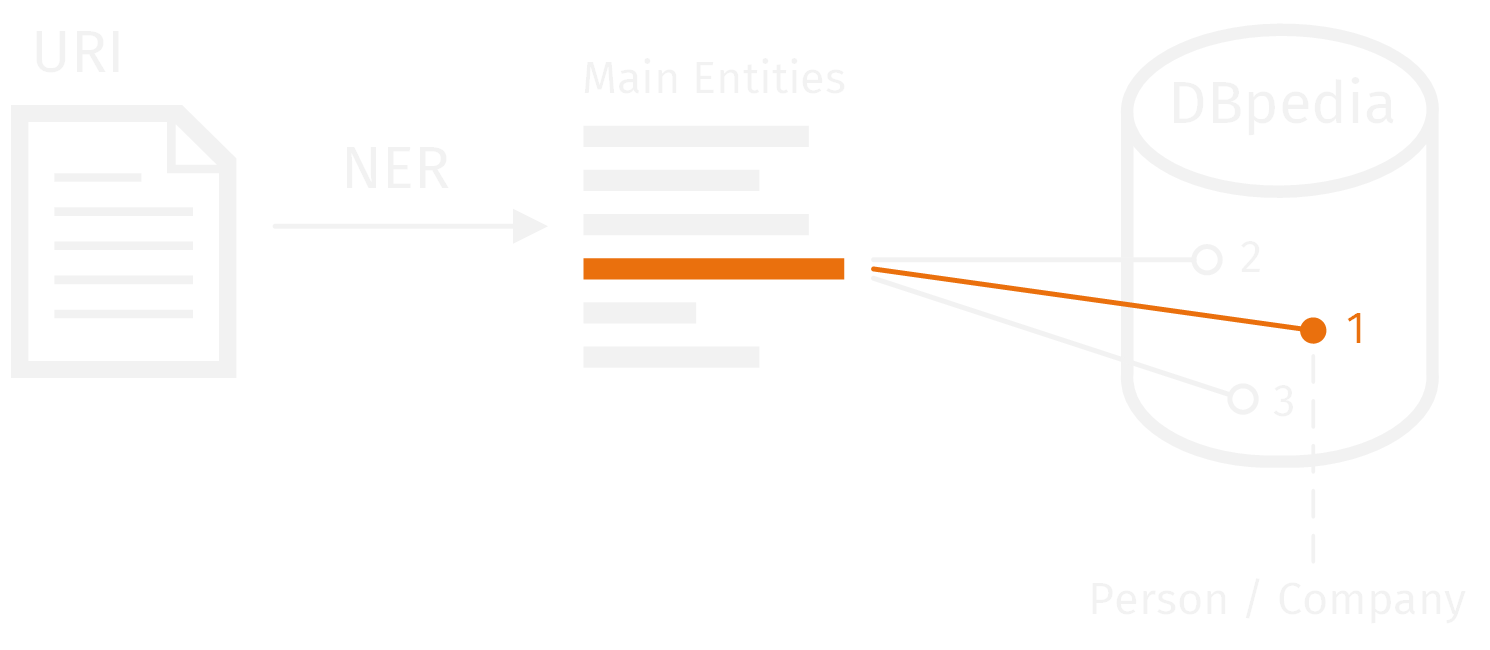
\includegraphics[width=.75\textwidth]{img/muddy_boots.png}
    \caption{How Muddy Boots works}
  \end{figure}

\end{frame}


% ------------------------------------------------------------------------------
\section{Content Link Tool}

\begin{frame}[fragile]{Content Link Tool}

  Annotation tool to manually edit metadata

  High quality automated suggestions

\end{frame}








% ===========================================================================================
% ===========================================================================================
% ===========================================================================================

% \section{Titleformats}

% \begin{frame}{Metropolis titleformats}
%     \themename supports 4 different titleformats:
%     \begin{itemize}
%         \item Regular
%         \item \textsc{Smallcaps}
%         \item \textsc{allsmallcaps}
%         \item ALLCAPS
%     \end{itemize}
%     They can either be set at once for every title type or individually.
% \end{frame}

% {
%     \metroset{titleformat frame=smallcaps}
% \begin{frame}{Small caps}
%     This frame uses the \texttt{smallcaps} titleformat.

%     \begin{alertblock}{Potential Problems}
%         Be aware, that not every font supports small caps. If for example you typeset your presentation with pdfTeX and the Computer Modern Sans Serif font, every text in smallcaps will be typeset with the Computer Modern Serif font instead.
%     \end{alertblock}
% \end{frame}
% }

% \begin{frame}{All small caps}
%     This frame uses the \texttt{allsmallcaps} titleformat.

%     \begin{alertblock}{Potential problems}
%         As this titleformat also uses smallcaps you face the same problems as with the \texttt{smallcaps} titleformat. Additionally this format can cause some other problems. Please refer to the documentation if you consider using it.

%         As a rule of thumb: Just use it for plaintext-only titles.
%     \end{alertblock}
% \end{frame}

% \begin{frame}{All caps}
%     This frame uses the \texttt{allcaps} titleformat.

%     \begin{alertblock}{Potential Problems}
%         This titleformat is not as problematic as the \texttt{allsmallcaps} format, but basically suffers from the same deficiencies. So please have a look at the documentation if you want to use it.
%     \end{alertblock}
% \end{frame}

% \section{Elements}

% \begin{frame}[fragile]{Typography}
%       \begin{verbatim}The theme provides sensible defaults to
% \emph{emphasize} text, \alert{accent} parts
% or show \textbf{bold} results.\end{verbatim}

%   \begin{center}becomes\end{center}

%   The theme provides sensible defaults to \emph{emphasize} text,
%   \alert{accent} parts or show \textbf{bold} results.
% \end{frame}

% \begin{frame}{Font feature test}
%   \begin{itemize}
%     \item Regular
%     \item \textit{Italic}
%     \item \textsc{SmallCaps}
%     \item \textbf{Bold}
%     \item \textbf{\textit{Bold Italic}}
%     \item \textbf{\textsc{Bold SmallCaps}}
%     \item \texttt{Monospace}
%     \item \texttt{\textbf{Monospace Bold}}
%   \end{itemize}
% \end{frame}

% \begin{frame}{Lists}
%   \begin{columns}[T,onlytextwidth]
%     \column{0.33\textwidth}
%       Items
%       \begin{itemize}
%         \item Milk \item Eggs \item Potatos
%       \end{itemize}

%     \column{0.33\textwidth}
%       Enumerations
%       \begin{enumerate}
%         \item First, \item Second and \item Last.
%       \end{enumerate}

%     \column{0.33\textwidth}
%       Descriptions
%       \begin{description}
%         \item[PowerPoint] Meeh. \item[Beamer] Yeeeha.
%       \end{description}
%   \end{columns}
% \end{frame}
% \begin{frame}{Animation}
%   \begin{itemize}[<+- | alert@+>]
%     \item \alert<4>{This is\only<4>{ really} important}
%     \item Now this
%     \item And now this
%   \end{itemize}
% \end{frame}
% \begin{frame}{Figures}
%   \begin{figure}
%     \newcounter{density}
%     \setcounter{density}{20}
%     \begin{tikzpicture}
%       \def\couleur{alerted text.fg}
%       \path[coordinate] (0,0)  coordinate(A)
%                   ++( 90:5cm) coordinate(B)
%                   ++(0:5cm) coordinate(C)
%                   ++(-90:5cm) coordinate(D);
%       \draw[fill=\couleur!\thedensity] (A) -- (B) -- (C) --(D) -- cycle;
%       \foreach \x in {1,...,40}{%
%           \pgfmathsetcounter{density}{\thedensity+20}
%           \setcounter{density}{\thedensity}
%           \path[coordinate] coordinate(X) at (A){};
%           \path[coordinate] (A) -- (B) coordinate[pos=.10](A)
%                               -- (C) coordinate[pos=.10](B)
%                               -- (D) coordinate[pos=.10](C)
%                               -- (X) coordinate[pos=.10](D);
%           \draw[fill=\couleur!\thedensity] (A)--(B)--(C)-- (D) -- cycle;
%       }
%     \end{tikzpicture}
%     \caption{Rotated square from
%     \href{http://www.texample.net/tikz/examples/rotated-polygons/}{texample.net}.}
%   \end{figure}
% \end{frame}

% \begin{frame}{Tables}
%   \begin{table}
%     \caption{Largest cities in the world (source: Wikipedia)}
%     \begin{tabular}{@{} lr @{}}
%       \toprule
%       City & Population\\
%       \midrule
%       Mexico City & 20,116,842\\
%       Shanghai & 19,210,000\\
%       Peking & 15,796,450\\
%       Istanbul & 14,160,467\\
%       \bottomrule
%     \end{tabular}
%   \end{table}
% \end{frame}

% \begin{frame}{Blocks}
%   Three different block environments are pre-defined and may be styled with an
%   optional background color.

%   \begin{columns}[T,onlytextwidth]
%     \column{0.5\textwidth}
%       \begin{block}{Default}
%         Block content.
%       \end{block}

%       \begin{alertblock}{Alert}
%         Block content.
%       \end{alertblock}

%       \begin{exampleblock}{Example}
%         Block content.
%       \end{exampleblock}

%     \column{0.5\textwidth}

%       \metroset{block=fill}

%       \begin{block}{Default}
%         Block content.
%       \end{block}

%       \begin{alertblock}{Alert}
%         Block content.
%       \end{alertblock}

%       \begin{exampleblock}{Example}
%         Block content.
%       \end{exampleblock}

%   \end{columns}
% \end{frame}
% \begin{frame}{Math}
%   \begin{equation*}
%     e = \lim_{n\to \infty} \left(1 + \frac{1}{n}\right)^n
%   \end{equation*}
% \end{frame}
% \begin{frame}{Line plots}
%   \begin{figure}
%     \begin{tikzpicture}
%       \begin{axis}[
%         mlineplot,
%         width=0.9\textwidth,
%         height=6cm,
%       ]

%         \addplot {sin(deg(x))};
%         \addplot+[samples=100] {sin(deg(2*x))};

%       \end{axis}
%     \end{tikzpicture}
%   \end{figure}
% \end{frame}
% \begin{frame}{Bar charts}
%   \begin{figure}
%     \begin{tikzpicture}
%       \begin{axis}[
%         mbarplot,
%         xlabel={Foo},
%         ylabel={Bar},
%         width=0.9\textwidth,
%         height=6cm,
%       ]

%       \addplot plot coordinates {(1, 20) (2, 25) (3, 22.4) (4, 12.4)};
%       \addplot plot coordinates {(1, 18) (2, 24) (3, 23.5) (4, 13.2)};
%       \addplot plot coordinates {(1, 10) (2, 19) (3, 25) (4, 15.2)};

%       \legend{lorem, ipsum, dolor}

%       \end{axis}
%     \end{tikzpicture}
%   \end{figure}
% \end{frame}
% \begin{frame}{Quotes}
%   \begin{quote}
%     Veni, Vidi, Vici
%   \end{quote}
% \end{frame}

% {%
% \setbeamertemplate{frame footer}{My custom footer}
% \begin{frame}[fragile]{Frame footer}
%     \themename defines a custom beamer template to add a text to the footer. It can be set via
%     \begin{verbatim}\setbeamertemplate{frame footer}{My custom footer}\end{verbatim}
% \end{frame}
% }

% \begin{frame}{References}
%   Some references to showcase [allowframebreaks] \cite{Kobilarov2009}
% \end{frame}

\section{Conclusion}

\begin{frame}{Conclusion}

  User experience in the center of efforts

  Smart interlinking to internal and external resources

  Well integrated and hidden systems

\end{frame}

\begin{frame}[standout]
  Thanks for your attention!

  \bigskip
  \alert{Questions?}
\end{frame}

\begin{frame}[allowframebreaks]{References}

  \nocite{*}
  \bibliography{references}
  \bibliographystyle{abbrv}

\end{frame}

\end{document}